\documentclass{article}
\usepackage[ backend=biber]{biblatex}
\addbibresource{prop.bib}
\ExecuteBibliographyOptions{sorting=nyt,maxbibnames=5,doi=false,isbn=false,url=false}
\usepackage{fullpage}
\usepackage[utf8]{inputenc}
\usepackage{tensor}
\usepackage{url}
\usepackage{amsmath}
\usepackage{amssymb}
\usepackage{amsthm}
\usepackage{mathrsfs}
\usepackage{bbm}
\usepackage{bbold}
\usepackage{wesa}
\usepackage{graphicx}

\theoremstyle{remark}
\newtheorem{example}{Example}
\newtheorem{definition}{Definition}
\newtheorem{cor}{Corollary}
\newtheorem{lemma}{Lemma}
\newtheorem{thm}{Theorem}
\newtheorem{case}{Case}
\newtheorem{conjecture}{Conjecture}
\newtheorem{problem}{Problem}
\newtheorem{claim}{Claim}

\newcommand{\Hilb}{\mathcal{H}}
\newcommand{\events}{\ensuremath{\mathcal{E}}}
\newcommand{\qevents}{\ensuremath{\mathcal{E}}}
\newcommand{\pmeas}{\ensuremath{\mu}}
\newcommand{\imposs}{{\mbox{\wesa{impossible}}}}
\newcommand{\likely}{{\mbox{\wesa{likely}}}}
\newcommand{\unlikely}{{\mbox{\wesa{unlikely}}}}
\newcommand{\necess}{{\mbox{\wesa{certain}}}}
\newcommand{\overflow}{{\mbox{\wesa{overflow}}}}
\newcommand{\unknown}{{\mbox{\wesa{unknown}}}}
\newcommand{\bra}[1]{{\left\langle{#1}\right\vert}}
\newcommand{\ket}[1]{{\left\vert{#1}\right\rangle}}
\newcommand{\op}[2]{\ensuremath{\left\vert{#1}\middle\rangle\middle\langle{#2}\right\vert}}
\newcommand{\proj}[1]{\op{#1}{#1}}
\def\C{{\mathbb{C}}}
\newcommand{\ps}{\texttt{+}}
\newcommand{\ms}{\texttt{-}}
\newcommand{\ip}[2]{\ensuremath{\left\langle{#1}\middle\vert{#2}\right\rangle}}
\newcommand{\Tr}{\mathop{\mathrm{Tr}}\nolimits}
\newcommand{\rme}{\mathrm{e}}
\newcommand{\rmi}{\mathrm{i}}

%% \title{Computational Quantum Probabilities}
%% \title{Measurement and Probability in Fuzzy Quantum Theories}
\title{Measurement and Probability in Fuzzy Quantum Theories}
\date{}
\begin{document}
\maketitle 

%%%%%%%%%%%%%%%%%%%%%%%%%%%%%%%%%%%%%%%%%%%%%%%%%%%%%%%%%%%%%%%%%%%%%%%%%%%%%%
\section{Overview, Objectives, and Expected Significance} 

This is a \emph{theoretical} investigation of \emph{experimental}
physics using \emph{computational} methods. All experiments and
computations are processes bounded in space, time, energy, and other
resources. Yet, for centuries, the mathematical formalization of such
processes has been founded on the infinitely precise real or complex
numbers. Indeed, almost every description of quantum mechanics,
quantum computation, or quantum experiments refers to entities such as
$e$, $\pi$, $\sqrt{2}$, etc. From a computational perspective, such
numbers do not exist in their entirety ``for free.''  For example, the
state of the art algorithms for computing the $n$th binary digit of~$\pi$
require on the order of $O(n\log^{O(1)}(n))$
operations~\cite{journals/moc/BaileyBP97}. In other words, simply
referring to the $n$th digit of $\pi$ requires more and more resources
as $n$ gets larger. Taking such resource bounds into consideration is
what founded computer science as a discipline and is crucial for
understanding the very nature of computation and, following
Feynman~\cite{Feynman1982Simulating}, Landauer~\cite{Landauer1996188},
and others, for understanding the very nature of physical processes.

We propose to revisit quantum mechanics, quantum information, and
quantum computation from this resource-aware perspective. Our initial
results in that domain showed how subtle the issues can be~\cite{usat}:
a straightforward replacement of the complex numbers by a finite field
yields a variant of quantum mechanics in which computationally hard
problems like UNIQUE-SAT (which decides whether a given Boolean
formula is unsatisfiable or has exactly one satisfying assignment) can
be deterministically solved in constant time. To eliminate such
unrealistic theories requires delicate analysis of the structure of
the Hilbert space, the process of observation, and the notion of
probability teasing apart their reliance on the infinitely precise
real numbers~\cite{geometry2013,DQT2014}. In this proposal, our aim is
to shift focus from the infinitely-specified but not directly
observable quantum states, to observable measurable properties of
quantum systems and their probabilities. Furthermore, we insist that
our theories of measurement and probability only refer to finitely
communicable evidence within feasible computational bounds. It follows
that states, observations, and probabilities all become ``fuzzy'',
i.e., specified by intervals of confidence that can only increase in
precision if the available resources increase proportionally. Our
notion of ``fuzzy quantum mechanics'' is related to existing
work~\cite{GranikCaulfield1996,Pykacz2013,SNL2009,Gudder2005,aerts1993physical}
but, as will be explained in more detail, is distinguished by its
computational character.

We will begin by reviewing existing work that recasts classical
probability spaces in a resource-aware setting and move to our
proposal which, briefly speaking, aims at recasting quantum
probability and hence quantum measurement to a corresponding
resource-aware setting. In particular, we plan on addressing the
Meyer-Mermin debate~\cite{PhysRevLett.83.3751, Mermin1999,
  BarrettKent2004} on the impact of finite precision measurements on
the relevance of the Kochen-Specker
theorem~\cite{kochenspecker1967,Redhead1987-REDINA,peres1995quantum,Jaeger2007}.
We argue that no matter what the results are their impact will be
strong. Positive results that formulate a computable, with clear
resource bounds, theory of quantum measurement and quantum probability
would be essential for understanding and realizing quantum
computation. Any negative results would redirect research that aims at
realizing quantum computation to other approaches. At an intellectual
level, the results have the potential to solve or clarify several
paradoxes in quantum mechanics, quantum information, computability,
and complexity theory.

%%%%%%%%%%%%%%%%%%%%%%%%%%%%%%%%%%%%%%%%%%%%%%%%%%%%%%%%%%%%%%%%%%%%%%%%%%%%%%
\section{Background I: Classical Probability}

A \emph{probability space} specifies the necessary conditions for
reasoning coherently about collections of uncertain
events~\cite{Kolmogorov1950,Shafer1976,Griffiths2003,Swart2013}.  We
review the conventional presentation of probability spaces and then
discuss the computational resources needed to estimate probabilities.

%%%
\subsection{Classical Probability Spaces}

The conventional definition of a probability space builds upon the
field of real numbers. In more detail, a probability space consists of
a \emph{sample space} $\Omega$, a space of \emph{events}~$\events$,
and a \emph{probability measure}~$\pmeas$ mapping events in $\events$
to the real interval $[0,1]$. We will only consider \emph{finite} sets
of events and restrict our attention to non-empty finite sets $\Omega$
as the sample space. The space of events $\events$ includes every
possible subset of $\Omega$: it is the
powerset~$2^{\Omega}=\left\{ E ~\middle|~ E\subseteq\Omega\right\}
$.
For future reference, we emphasize that events are the primary notion
of interest and that the sample space is a convenient artifact that
allows us to treat events as sets obeying the laws of Boolean
algebra~\cite{Boole1948,Redhead1987-REDINA,Griffiths2003}.

\begin{definition}[Probability Measure]\label{def:ClassicalProbabilitySpace}
  Given the set of events $\events$, a \emph{probability measure} is a
  function $\pmeas:\events\rightarrow[0,1]$ such that:
\begin{itemize}
\item $\pmeas(\emptyset)=0$,
\item $\pmeas(\Omega)=1$, 
\item for every event $E$,
  $\pmeas\left(\Omega\backslash E\right)=1-\pmeas\left(E\right)$ where
  $\Omega\backslash E$ is the complement event of $E$, and
\item for every collection $\left\{ E_{i}\right\} _{i=1}^{N}$ of
  pairwise disjoint events,
  $\pmeas\left(\bigcup_{i=1}^{N}E_{i}\right)=\sum_{i=1}^{N}\pmeas(E_{i})$.
\end{itemize}
\end{definition}
\noindent There is some redundancy in the definition that will be useful when
moving to quantum probability spaces. 

\begin{example}[Two-coins experiment]\label{ex1} Consider an
  experiment that tosses two coins. We have four possible outcomes
  that constitute the sample space $\Omega=\{HH,HT,TH,TT\}$. There are
  16 total events including the event $\{HH,HT\}$ that the first coin
  lands heads up, the event $\{HT,TH\}$ that the two coins land on
  opposite sides, and the event $\{HT,TH,TT\}$ that at least one coin
  lands tails up. Here is a possible probability measure for these
  events:
\[
\begin{array}{c@{\qquad\qquad}c}
\begin{array}{rcl}
\pmeas(\emptyset) & = & 0\\
\pmeas(\{HH\}) & = & 1/3\\
\pmeas(\{HT\}) & = & 0\\
\pmeas(\{TH\}) & = & 2/3\\
\pmeas(\{TT\}) & = & 0\\
\pmeas(\{HH,HT\}) & = & 1/3\\
\pmeas(\{HH,TH\}) & = & 1\\
\pmeas(\{HH,TT\}) & = & 1/3
\end{array} & \begin{array}{rcl}
\pmeas(\{HT,TH\}) & = & 2/3\\
\pmeas(\{HT,TT\}) & = & 0\\
\pmeas(\{TH,TT\}) & = & 2/3\\
\pmeas(\{HH,HT,TH\}) & = & 1\\
\pmeas(\{HH,HT,TT\}) & = & 1/3\\
\pmeas(\{HH,TH,TT\}) & = & 1\\
\pmeas(\{HT,TH,TT\}) & = & 2/3\\
\pmeas(\{HH,HT,TH,TT\}) & = & 1
\end{array}\end{array}
\]
\end{example}

\noindent It is useful to think that this probability measure is
completely determined by the ``reality'' of the two coins in question
and their characteristics, in the sense that each pair of coins
induces a measure, and each measure must correspond to some pair of
coins. The measure above would be induced by two particular coins such
that the first coin is twice as likely to land tails up than heads up
and the second coin is double-headed. In a strict computational
or experimental setting, one should question the reliance of the
definition of probability space on the uncountable and
uncomputable real
interval~$[0,1]$~\cite{Turing_1937,Ziegler2007,weihrauch2012computable}.
This interval includes numbers like
$0.h_{1}h_{2}h_{3}\ldots$ where $h_{i}$ is 1 or 0 depending on whether
Turing machine $M_{i}$ halts or not. Such numbers cannot be
computed. This interval also includes numbers like $\frac{\pi}{4}$
which can only be computed with increasingly large resources as the
precision increases. Therefore, in a resource-aware computational or
experimental setting, it is more appropriate to consider probability
measures that map events to a set of elements computable with a fixed
set of resources. We expand on this observation in the next section
and then recall its formalization using interval-valued probability
measures~\cite{Weichselberger2000,JamisonLodwick2004}.

%%%%%
\subsection{Measuring Probabilities: Buffon's Needle Problem\label{subsec:Measuring-Probabilities:-Buffon}}

In the previous example, we assumed the probability~$\pmeas(E)$ of
each event~$E$ is known a priori. In reality, although each event is
assumed to have a probability, the exact value of $\pmeas(E)$ may not
be known. According to the \emph{frequency interpretation of
  probability} (which we will revisit when moving to the quantum
case)~\cite{Venn1876,Hajek2012}, 
to determine the probability of an event, we run $N$
independent trials which gives us an approximation of the (assumed)
``true'' or ``real'' probability. Let $x_{i}$ be 1 or 0 depending on
whether the event~$E$ occurs in the $i$-th trial or not, then
$\pmeas(E)$ could be approximated to given accuracy~$\epsilon>0$ by
the relative frequency~$\frac{1}{N}\sum_{i=1}^{N}x_{i}$ with the
probability converging to one as $N$ goes to infinity, i.e.,
\[
\forall\epsilon>0,\lim_{N\rightarrow\infty}\pmeas\left(\left|\pmeas(E)-\frac{1}{N}\sum_{i=1}^{N} x_{i}\right|<\epsilon\right)=1\textrm{ .}
\]
This fact is called the law of large numbers~\cite{Bernoulli2006,Kolmogorov1950,Uspensky1937,Shafer1976,544199}.

Let's look at a concrete example. Suppose we drop a needle of length
$\ell$ onto a floor made of equally spaced parallel lines a distance
$h$ apart, where $\ell<h$. It is a known fact that the probability of
the needle crossing a line is
$\frac{2\ell}{\pi
  h}$~\cite{Buffon1777,DeMorgan1872,Hall1873,Uspensky1937}.
Consider an experimental setup consisting of a collection of $N$
identical needles of length $\ell$. We throw the $N$ needles one
needle at a time, and observe the number $M$ of needles that cross a
line, thus estimating the probability of a needle crossing a line to
be $\frac{M}{N}$. In an actual experiment with $500$ needles and the
ratio $\frac{\ell}{h}=0.75$~\cite{Hall1873}, it was found that $236$
crossed a line so the relative frequency is $0.472$ whereas the
idealized mathematical probability is $0.4774\ldots$.  In a larger
experiment with $5000$ needles and the ratio
$\frac{\ell}{h}=0.8$~\cite{Uspensky1937}, the relative frequency was
calculated to be $0.5064$ whereas the idealized mathematical
probability is $0.5092\ldots$. We see that the observed probability
approaches $\frac{2\ell}{\pi h}$ but only if \emph{larger and larger
  resources} are expended. These resource considerations suggest that
it is possible to replace the real interval $[0,1]$ with rational
numbers up to a certain precision related to the particular experiment
in question. There is clearly a connection between the number of
needles and the achievable precision: in the hypothetical experiment
with 3 needles, it is not sensible to retain 100 digits in the
expansion of $\frac{2\ell}{\pi h}$.

There is another more subtle assumption of unbounded computational
power in the experiment. We are assuming that we can always determine
with certainty whether a needle is crossing a line. But ``lines'' on
the the floor have thickness, their distance apart is not exactly $h$,
and the needles' lengths are not all absolutely equal to $\ell$.
These perturbations make the events ``fuzzy.'' Thus, in an experiment
with limited resources, it is not possible to talk about the idealized
event that exactly $M$ needles cross lines as this would require the
most expensive needles built to the most precise accuracy, laser
precision for drawing lines on the floor, and the most powerful
microscopes to determine if a needle does cross a line. Instead we
might talk about the event that $M-\delta$ needles evidently cross
lines and $M+\delta'$ needles plausibly cross lines where $\delta$ and
$\delta'$ are resource-dependent approximations. This fuzzy notion of
events leads to probabilities being only calculable within intervals
of confidence reflecting the certainty of events and their
plausibility. This is indeed consistent with published experiments: in
an experiment with $3204$ needles and the ratio
$\frac{\ell}{h}=0.6$~\cite{DeMorgan1872}, $1213$ needles clearly
crossed a line and $11$ needles were close enough to plausibly be
considered as crossing the line: we would express the probability in
this case as the interval
$\left[\frac{1213}{3204},\frac{1224}{3204}\right]$ expressing that we
are certain that the event has probability at least
$\frac{1213}{3204}$ but it is possible that it would have probability
$\frac{1224}{3204}$.

%%%%%
\subsection{Classical Interval-Valued Probability Measures}

As motivated above, an event $E_{1}$ may have an interval of
probability $[l_{1},r_{1}]$. Assume that another disjoint event
$E_{2}$ has an interval of probability $[l_{2},r_{2}]$, what is the
interval of probability for the event $E_{1}\cup E_{2}$? The answer is
somewhat subtle: although it is possible to use the sum of the
intervals $[l_{1}+l_{2},r_{1}+r_{2}]$ as the combined probability, one
can find a much tighter interval if information \emph{against} the
event (i.e., information about the complement event) is also taken
into consideration. Formally, for a general event $E$ with probability
$[l,r]$, the evidence that contradicts $E$ is evidence supporting the
complement of $E$.  The complement of $E$ must therefore have
probability $\left[1-r,1-l\right]$ which we abbreviate
$\left[1,1\right]-\left[l,r\right]$.  Given a sample space~$\Omega$
and its set of events~$\events$, a
function~$\bar{\mu}:\events\rightarrow[0,1]$ is a classical
interval-valued probability measure if and only if $\bar{\mu}$
satisfies the following conditions~\cite{JamisonLodwick2004} where the
last line uses $\subseteq$ to allow for tighter intervals that exploit
the complement event:
\begin{itemize}
\item $\bar{\mu}(\emptyset)=[0,0]$.
\item $\bar{\mu}(\Omega)=[1,1]$. 
\item For any event $E$,
  $\bar{\mu}\left(\Omega\backslash E\right)=\left[1,1\right]-\bar{\mu}\left(E\right)$
\item For a collection $\left\{ E_{i}\right\} _{i=1}^{N}$ of pairwise
  disjoint events, we have
  $\bar{\mu}\left(\bigcup_{i=1}^{N}E_{i}\right)\subseteq\sum_{i=1}^{N}\bar{\mu}\left(E_{i}\right)$.
\end{itemize}

\begin{example}[Two-coin experiment with interval probability]
\label{ex3} We split the unit interval $[0,1]$ in the following
four closed sub-intervals: $[0,0]$ which we call \imposs, $[0,\frac{1}{2}]$
which we call \unlikely, $[\frac{1}{2},1]$ which we call \likely,
and $[1,1]$ which we call \necess. Using these new values, we can
modify the probability measure of Ex.~\ref{ex1} by mapping each
numeric value to the smallest sub-interval containing it to get the
following: 
\[
\begin{array}{c@{\qquad\qquad}c}
\begin{array}{rcl}
\bar{\mu}(\emptyset) & = & \imposs\\
\bar{\mu}(\{HH\}) & = & \unlikely\\
\bar{\mu}(\{HT\}) & = & \imposs\\
\bar{\mu}(\{TH\}) & = & \likely\\
\bar{\mu}(\{TT\}) & = & \imposs\\
\bar{\mu}(\{HH,HT\}) & = & \unlikely\\
\bar{\mu}(\{HH,TH\}) & = & \necess\\
\bar{\mu}(\{HH,TT\}) & = & \unlikely
\end{array} & \begin{array}{rcl}
\bar{\mu}(\{HT,TH\}) & = & \likely\\
\bar{\mu}(\{HT,TT\}) & = & \imposs\\
\bar{\mu}(\{TH,TT\}) & = & \likely\\
\bar{\mu}(\{HH,HT,TH\}) & = & \necess\\
\bar{\mu}(\{HH,HT,TT\}) & = & \unlikely\\
\bar{\mu}(\{HH,TH,TT\}) & = & \necess\\
\bar{\mu}(\{HT,TH,TT\}) & = & \likely\\
\bar{\mu}(\{HH,HT,TH,TT\}) & = & \necess
\end{array}\end{array}
\]
Despite the absence of infinitely precise numeric information, the
probability measure is quite informative: it reveals that the second
coin is double-headed and that the first coin is biased. To understand
the $\subseteq$-condition, consider the following calculation:
\begin{eqnarray*}
\bar{\mu}(\{HH\})+\bar{\mu}(\{HT\})+\bar{\mu}(\{TH\})+\bar{\mu}(\{TT\})
&=& \imposs+\unlikely+\imposs+\likely\\
&=& \left[0,0\right]+\left[0,\frac{1}{2}\right]+\left[0,0\right]+\left[\frac{1}{2},1\right]\\
&=& \left[\frac{1}{2},\frac{3}{2}\right]
\end{eqnarray*}
If we were to equate $\bar{\mu}(\Omega)$ with the sum of the individual
probabilities, we would get that $\bar{\mu}(\Omega)=\left[\frac{1}{2},\frac{3}{2}\right]$.
However, using the fact that $\bar{\mu}(\emptyset)=\imposs$, we have
$\bar{\mu}\left(\Omega\right)=1-\bar{\mu}\left(\emptyset\right)=\necess=[1,1]$.
This interval is tighter and a better estimate for the probability
of the event $\Omega$, and of course it is contained in $[\frac{1}{2},\frac{3}{2}]$.
However it is only possible to exploit the information about the complement
when all four events are combined. Thus the $\subseteq$-condition
allows us to get an estimate for the combined event from each of its
constituents and then gather more evidence knowing the aggregate
event.
\end{example}

%%%%%%%%%%%%%%%%%%%%%%%%%%%%%%%%%%%%%%%%%%%%%%%%%%%%%%%%%%%%%%%%%%%%%%%%%%%%%%
\section{Background II: Quantum Probability}
 
The mathematical framework of classical probability above assumes that
there exists a predetermined set of events that are independent of the
particular experiment --- classical physics is
non-contextual~\cite{kochenspecker1967,Redhead1987-REDINA,peres1995quantum,Jaeger2007}. 
However, even in classical situations, the structure
of the event space is often only partially known and the precise
dependence of two events on each other cannot, a priori, be determined
with certainty. In the quantum framework, this partial knowledge is
compounded by the fact that there exist non-commuting events which
cannot happen simultaneously. To accommodate these more complex
situations, conventional approaches to quantum probability abandon the
sample space~$\Omega$ and reason directly about events which are
generalized from plain sets to projection operators. A quantum
probability space therefore consists of just two components: a set of
events $\qevents$ often formalized as projection operators and a
probability measure $\mu:\qevents\rightarrow[0,1]$ formalized using
the Born rule~\cite{Born1983,Mermin2007,Jaeger2007}.

%%%%%
\subsection{Quantum Events}

\begin{definition}[Projection Operators; Orthogonality~\cite{10.2307/2308516,Redhead1987-REDINA,peres1995quantum,Griffiths2003,Swart2013}]
  \label{def:Projection} Given a Hilbert space $\Hilb$, an event (an
  experimental proposition~\cite{BirkhoffVonNeumann1936}, a
  question~\cite{10.2307/2308516,Abramsky2012},
  or an elementary quantum test~\cite{peres1995quantum}) is represented
  as a (self-adjoint or orthogonal~\cite {Griffiths2003,Maassen2010})
  projection operator $P:\Hilb\rightarrow\Hilb$ onto a linear subspace
  of $\Hilb$. The following define projections and list some of their properties:
\begin{itemize}
\item $\mathbb{0}$ is a projection. 
\item For any pure state~$\ket{\psi}$, $\proj{\psi}$ is a projection
operator. 
\item Projection operators $P_{0}$ and $P_{1}$ are \emph{orthogonal}
  if $P_{0}P_{1}=P_{1}P_{0}=\mathbb{0}$. The sum of two projection
  operators~$P_{0}+P_{1}$ is also a projection operator if and only if
  they are orthogonal.
\item Conversely, every projection~$P$ can be expressed as
  $\sum_{j=1}^{N}\proj{\psi_{j}}$, where $P$ actually projects onto
  the linear subspace with orthonormal
  basis~$\left\{ \ket{\psi_{j}}\right\} _{j=1}^{N}$.
\item A set of projections $\left\{ P_{i}\right\} _{i=1}^{N}$ is
  called an \emph{ideal measurement} if it is a partition of the
  identity, i.e., $\sum_{i=1}^{N}P_{i}=\mathbb{1}$~\cite{Swart2013}.
  In this case, projections $\left\{ P_{i}\right\} _{i=1}^{N}$ must
  be mutually orthogonal~\cite{Griffiths2003,Halmos1957}, and $N$ must be less
  or equal to the dimension of the Hilbert space.
\item If $P$ is a projection operator, then $\mathbb{1}-P$ is also a
  projection operator, called its \emph{complement}. It is orthogonal to
  $P$, and corresponds to the complement event~$\Omega\backslash E$ in
  classical probability~\cite{Griffiths2003}.
\item Projection operators $P_{0}$ and $P_{1}$ \emph{commute} if $P_{0}P_{1}=P_{1}P_{0}$.
The product of two projection operators~$P_{0}P_{1}$ is also a projection
operator if and only if they commute. This corresponds to the classical
intersection between events~\cite{peres1995quantum,Griffiths2003}. 
\item For two commuting projection operators $P_{0}$ and $P_{1}$,
  their \emph{disjunction}~$P_{0}\vee P_{1}$ is defined to be
  $P_{0}+P_{1}-P_{0}P_{1}$~\cite{Griffiths2003}.
\end{itemize}
\end{definition}

\begin{example}[One-qubit quantum probability space] Consider a
  one-qubit Hilbert space with each event interpreted as a possible
  post-measurement state~\cite{peres1995quantum,Mermin2007,Jaeger2007}. 
  For example, the event $\proj{0}$ indicates
  that the post-measurement state will be $\ket{0}$; the probability
  of such an event depends on the current state; the event $\proj{1}$
  indicates that the post-measurement state will be $\ket{1}$; the
  event $\proj{\ps}$ where
  $\ket{\ps}=\frac{1}{\sqrt{2}}(\ket{0}+\ket{1})$ indicates that the
  post-measurement state will be $\ket{\ps}$; the event
  $\mathbb{1}=\proj{0}+\proj{1}$ indicates that the post-measurement
  state will be a linear combination of $\ket{0}$ and $\ket{1}$ and is
  clearly certain; finally the empty event $\mathbb{0}$ states that
  the post-measurement state will be the empty state and is
  impossible. As in the classical case, a probability measure is a
  function that maps events to $[0,1]$. Here is a partial
  specification of a possible probability measure that would be
  induced by a system whose current state is $\ket{0}$,
  $\mu\left(\mathbb{0}\right)=0$, $\mu\left(\mathbb{1}\right)=1$,
  $\mu\left(\proj{0}\right)=1$, $\mu\left(\proj{1}\right)=0$,
  $\mu\left(\proj{\ps}\right)=1/2$, \ldots. Note that, similarly to
  the classical case, the probability of $\mathbb{1}$ is 1 and the
  probability of collections of orthogonal events (e.g.,
  $\proj{0}+\proj{1}$) is the sum of the individual probabilities.  A
  collection of non-orthogonal events (e.g., $\proj{0}$ and
  $\proj{\ps}$) is however not even a valid event. In the classical
  example, we argued that each probability measure is uniquely
  determined by two actual coins. A similar (but much more subtle)
  argument is valid also in the quantum case. By postulates of quantum
  mechanics and Gleason's theorem, it turns out that for large enough
  quantum systems, each probability measure is uniquely determined by
  an actual quantum state as discussed next.
\end{example}

%%%%%
\subsection{Quantum Probability Measures}

Given our setup, the definition of a quantum probability measure is a
small variation on the classical definition. 

\begin{definition}[Quantum Probability Measure~\cite{10.2307/2308516,gleason1957,Redhead1987-REDINA,Maassen2010}]\label{def:QuantumProbabilitySpace}
Given a Hilbert space $\Hilb$ with its set of events~$\events$,
a \emph{quantum probability measure} is a function~$\mu:\events\rightarrow[0,1]$
such that: 
\begin{itemize}
\item $\mu(\mathbb{0})=0$. 
\item $\mu(\mathbb{1})=1$. 
\item For any projection $P$, $\mu\left(\mathbb{1}-P\right)=1-\mu\left(P\right)$.
\item For a set of mutually orthogonal projections $\left\{ P_{i}\right\} _{i=1}^{N}$,
we have $\mu\left(\sum_{i=1}^{N}P_{i}\right)=\sum_{i=1}^{N}\mu\left(P_{i}\right)$.
\end{itemize}
\end{definition}

\noindent A quantum probability measure can be easily constructed if
one knows the current state of the quantum system by using the Born
rule.  Specifically, for each
pure normalized quantum state $\ket{\phi}$, the Born rule induces a
probability measure $\mu_{\phi}^{B}$ defined as
$\mu_{\phi}^{B}(P)=\ip{\phi}{P\phi}$. The situation generalizes to
mixed states $\rho = \sum_{j=1}^{N}q_{j}\proj{\phi_{j}}$, where
$\sum_{j=1}^{N}q_{j}=1$ in which case the generalized Born rule
induces a probability measure $\mu_{\rho}^{B}$ defined
as
$\mu_{\rho}^{B}\left(P\right) = \Tr\left(\rho P\right) =
\sum_{j=1}^{N}
q_{j}\mu_{\phi_{j}}^{B}\left(P\right)$~\cite{peres1995quantum,544199,Jaeger2007}.
Conversely every probability measure must be of this form.

\begin{thm}[Gleason's
  theorem~\cite{gleason1957,Redhead1987-REDINA,peres1995quantum}]\label{cor:Gleason's}In
a Hilbert space $\Hilb$ of dimension $d\geq3$, given a quantum probability
measure~$\mu:\events\rightarrow[0,1]$, there exists a unique mixed
state~$\rho$ such that $\mu=\mu_{\rho}^{B}$.
\end{thm}

%%%%%
\subsection{Measuring Quantum Probabilities}

Similarly to the classical case, it is possible to estimate quantum
probabilities by utilizing the frequentist approach of the previous
section, assuming identical measurements conditions in each repeated
experiment~\cite{peres1995quantum}. 
For instance, if one wants to determine the probability
that the spin of a given silver atom is $+\hbar/2$, a Stern-Gerlach
apparatus is built where ideally an inhomogeneous magnetic field is
generated along, let's say, the quantization axis $z$. One then
produces a collimated beam of identically prepared (neutral) silver
atoms that is directed between the poles of the magnet where a
predetermined field-gradient along the $z$ direction has been
established. Under appropriate experimental conditions we will observe
that the beam, after traversing the magnetic-field region, will be
deflected towards two regions identified by distinguished spots on a
detector situated behind the
apparatus~\cite{Stern1988,peres1995quantum,544199,Griffiths2003}.
Each of the two discrete values is associated to either $+\hbar/2$ or
$-\hbar/2$, commonly called ``spin up'' and ``spin down'',
respectively. By ``counting'' the number of atoms that are deflected
in the ``spin up'' region one can, in principle, estimate the
probability that the prepared state of the silver atom state has spin
$+\hbar/2$. Notice that a real experiment does not necessarily
represent an ``ideal measurement''. For example, not all silver atoms
will be identically prepared, or the field-gradient could not be large
enough to distinguish between the spin up and down situations simply
producing a large single blot. In other words, the closer we get to an
ideal measurement the better we determine those probabilities at the
cost of significantly increasing the number of resources. It is not
very well appreciated in the literature that Bohr attempted to argue
against the measurability of the spin of a free electron. Essentially,
Bohr argued (and Mott later on justified his assertion by an elegant
use of uncertainty relations~\cite{10.2307/j.ctt7ztxn5.15}) that a
Stern-Gerlach experiment could not succeed in establishing the spin of
an unbound electron because the Lorentz force would blur the detected
pattern. This example illustrates the case of a fundamental physical
limitation that not even infinite resources could mitigate.

%%%%%%%%%%%%%%%%%%%%%%%%%%%%%%%%%%%%%%%%%%%%%%%%%%%%%%%%%%%%%%%%%%%%%%%%%%%%%%
\section{Proposal: General Plan} 

A major aim of this proposal is to recast quantum probability and
measurement in a computational resource-aware setting. Our vision is
to unify the strands above in a novel way as explained in this
section. We start with some immediate observations that justify the
rest of the development. 

\begin{itemize}

\item If we insist that probabilities cannot be infinitely precise and
  are bound to be approximations represented by intervals of
  confidence, then quantum states themselves cannot be infinitely precise
  because Gleason's theorem is no longer applied. 
  This raises an important philosophical
  question with immense practical relevance in the context of quantum
  computing. The question, which we could largely bypass in the
  classical case, is whether there is, in the background of all the
  measurements and probabilities, a ``real'' infinitely-precise
  quantum state that is being approximated and that, in principle, can
  be more and more accurately described given more and more
  resources. In other words, does a Gleason,
  Bell~\cite{BellBook1987,Redhead1987-REDINA,peres1995quantum,Jaeger2007}, 
  or Kochen-Specker
  theorem still hold in a world with finite resources?  The answer
  will have to be \emph{no} if we are to respect these major theorems
  of quantum mechanics and quantum information. Thus our first radical
  departure from the conventional case will be that the quantum state
  itself must be fuzzy in some sense to be formalized.

\item Going further we actually have to concede not just the infinite
  accuracy of the quantum state, but its very existence as a ``real''
  entity that exists independently of measurements and
  probabilities. The reasons for this second radical position are as
  follows. First arguments embedded in the proof of the Kochen-Specker
  theorem essentially rule out the existence of a sample space as the
  probabilities of events cannot be consistently expressed using core
  assignments to elements of the sample space. Second, the frequency
  interpretation of probability which is already problematic in the
  classical case, becomes untenable in the quantum case. In both
  cases, but much more in the quantum case, it is much more sensible
  to interpret probability in the Bayesian sense as ``lack of
  knowledge''. This, and similar arguments elegantly expressed by
  recent work on Quantum Bayesianism~\cite{Fuchs2010,VonBaeyer2016,Fuchs2012},
  suggest that the quantum state is more like an interactive system in
  computer science parlance. In other words, the state is only
  determined by its interactions with the environment or observers. A
  rough but useful analogy in the context of computer science would be
  a web server: the state of such a system cannot be said to exist
  independently of the interactions with clients; each interaction
  with a client determines a future state of the system and may affect
  future interactions. Crucially, each client may have a
  \emph{different} view of the web server that is consistent with
  their own history of interactions. This computational perspective
  agrees with the philosophical position of QBism~\cite{VonBaeyer2016}
  that asserts that the quantum state is subjective: each observer has
  a different view of the quantum system that is consistent with their
  previous observations and that allows that observer, independently
  of other observers, to assign beliefs (i.e., probabilities) to
  possible future interactions.

\end{itemize} 

%%%%
\subsection{Proposed Activity I: Quantum States as Interactive Processes} 

The early formalization of the process of computing using Turing
machines~\cite{Turing_1937,blum2012complexity} or the
$\lambda$-calculus~\cite{Church1932,Barendregt:Lambda} viewed a computation as
realizing a mathematical function. From our perspective, the most
important consequence of this view is that the properties of the
computed function existed independently of any observation,
calculation, or interaction. For example, a function is
\emph{injective} or not independently of any observation. An agent can
only interact with the computation by asking questions regarding its
input-output behavior and although such interaction would reveal
fragments of the computed function and its innate properties it could
not change it or affect it in any way.

In a series of breakthrough papers that led to his Turing
Award~\cite{Milner:1993:EIT:151233.151240}, Milner argued that this
``closed system'' view of computation is too limiting as it cannot
adequately describe the increasingly pervasive \emph{interactive
  computations}. Milner explained that ``concurrency requires a new
conceptual framework'' and ``not merely an extension of the repertoire
of entities and constructions which explain sequential computing.'' In
his Turing Award lecture, he gives the following simple but compelling
example. Consider the following two programs:
\begin{verbatim}
Program P1: x := 1; x := x + 1 
Program P2: x := 2
\end{verbatim}
As closed systems, these two programs define the same relation, namely
the one that maps an input memory to an updated memory in which the
location named \verb|x| is assigned the value \verb|2|. An observer
with the ability of inquire about the value of \verb|x| at the end of
the computation cannot distinguish the two programs. But place the
programs in an environment which may involve interactions and the
equivalence is lost. Phrased in physical terms, we give the observer the
additional ability to access the location \verb|x| \emph{during} the
computation, not just to observe its final value. In computing terms,
we place each of the two programs \verb|P1| and \verb|P2| concurrently
with the program:
\begin{verbatim}
Program Q: x := 3
\end{verbatim}
In the combined system of \verb|P1| and \verb|Q| running concurrently,
the location \verb|x| may end up containing \verb|2|, \verb|3|, or
\verb|4|. But in the combined system of \verb|P2| and \verb|Q| running
concurrently, the location~\verb|x| can only end up containing
\verb|2| or \verb|3|. The lesson, phrased in physics terms, is that it
is not sensible to think of the properties of a system (like \verb|P1|
or \verb|P2|) independently of the observer (\verb|Q| in this
case). Indeed the observation \verb|x=4| cannot be said to have an
existence independently from the interaction between \verb|P1| and
\verb|Q|: it really emerges or is created as part of the observation
process and is not a pre-existing ``element of reality''.

This phenomenon is hardly a surprise to computer scientists or
physicists but embracing it fully does have far-reaching
consequences. In computer science, the big shift was to abandon the
idea that a computation has inherent internal meaning, e.g.,
representing a pure mathematical function. Instead \emph{the meaning
  of a computational process is its observable behavior.} In this
computational analogue to the theory of controlled open quantum
systems, it is not too difficult to imagine that, in the presence of
multiple interacting observers, the behavior observed by just one
agent would appear to involve hidden variables or action at a
distance. The well-established theory of observation of concurrent
processes and their equivalences~\cite{Hennessy1989} relies on
neither.

\paragraph*{Research Question.} Is it possible to adapt the theory of
observation of concurrent processes to the study of quantum states and
confirm that the observations exhibit the same Bell-like correlations?

\paragraph*{Research Question.} The theory of observation of
concurrent processes and the theory of measurement in quantum
mechanics are superficially different. Is it possible to reformulate
them in a common language to benefit each theory from insights derived
from the other theory?

\paragraph*{Research Question.} Does the computational and hence
\emph{testable} hypothesis that the quantum state is nothing but an
interactive system agree with the QBism perspective providing a
resolution to the same paradoxes (e.g., EPR~\cite{EPR1935} and Wigner's
friend~\cite{Wigner1961,Fuchs2010,Fuchs2012})?

%%%%%
\subsection{Proposed Activity II: Quantum Interval-valued Probability Measures}
 
This is the most developed part of our current investigation and is
presented in greater detail than the other proposed activities. It
relies on current unpublished results. As argued in the previous
sections, given fixed finite resources, it is only possible to
estimate the quantum probabilities within an interval of
confidence. It is therefore natural to propose the notion of a
``quantum interval-valued probability measure'' that combines the
definitions of conventional quantum probability measures with
classical interval-probabilities.

\begin{definition}[Quantum Interval-valued Probability Measure]\label{def:QuantumInterval-valuedProbability}
  Given a Hilbert space $\Hilb$ with quantum events
  (projections)~$\events$, and a collection of
  intervals~$\mathscr{I}$, a \emph{quantum
    $\mathscr{I}$-interval-valued probability measure} is a
  function~$\bar{\mu}:\events\rightarrow\mathscr{I}$ such that:
\begin{itemize}
\item $\bar{\mu}(\mathbb{0})=\left[0,0\right]$. 
\item $\bar{\mu}(\mathbb{1})=\left[1,1\right]$. 
\item For any projection $P$,
  $\bar{\mu}\left(\mathbb{1}-P\right)=\left[1,1\right]-\bar{\mu}\left(P\right)$.
\item For a set of mutually orthogonal projections
  $\left\{ P_{i}\right\} _{i=1}^{N}$, we have
  $\bar{\mu}\left(\sum_{i=1}^{N}
    P_{i}\right)\subseteq\sum_{i=1}^{N}\bar{\mu}\left(P_{i}\right)$.
\end{itemize}
\end{definition}

\noindent It is easy to establish that quantum interval-valued
probability measures generalize conventional quantum probability
measures. In particular, any quantum probability measure can be recast
as an interval-valued measure using the three intervals
$\left[0,0\right]$, $\left[1,1\right]$ and \emph{$\left[0,1\right]$},
where $\left[0,0\right]$ and $\left[1,1\right]$ are called \imposs~and
\necess~as before, and \emph{$\left[0,1\right]$} is called
\unknown~because it provides no information. Given a quantum
probability measure~$\mu:\events\rightarrow\left[0,1\right]$, we
define a quantum interval-valued probability
measure~$\bar{\mu}:\events\rightarrow\mathscr{I}$ by
$\bar{\mu}(P)=\iota\left(\mu(P)\right)$, where
$\iota:\left[0,1\right]\rightarrow\mathscr{I}$ is defined by
\[
\iota(x)=\begin{cases}
\necess & \textrm{if }x=1\textrm{ ;}\\
\imposs & \textrm{if }x=0\textrm{ ;}\\
\unknown & \textrm{otherwise.}
\end{cases}
\]
This measure represents the beliefs of an experimenter with no prior 
knowledge about the particular quantum system in question. Formally,
we can ask: what can we deduce about the state of a quantum system
given a quantum interval-valued probability measure, i.e., given
observations done with finite resources. In the case the intervals are
infinitely precise the question reduces to Gleason's theorem which
states that the state of the quantum system is uniquely determined by
the probability measure. But surely the less resources are available,
the less precise the intervals, and the less we expect to know about
the state of the system. To formally state and answer this question we
begin with defining the \emph{core} and \emph{convexity} of a
probability measure as follows.

\begin{definition}
  Given a quantum interval-valued probability
  measure~$\bar{\mu}:\events\rightarrow\mathscr{I}$:
\begin{itemize}
\item A \emph{core} of $\bar{\mu}$ is the set
  $\mathrm{core}\left(\bar{\mu}\right)=\left\{
    \pmeas:\events\rightarrow[0,1] ~\middle|~ \forall
    E\in\events.~\pmeas\left(E\right)\in\bar{\mu}\left(E\right)\right\}$.
\item $\bar{\mu}$ is called convex if
  $\bar{\mu}\left(P_{0}\vee
    P_{1}\right)+\bar{\mu}\left(P_{0}P_{1}\right)\subseteq\bar{\mu}\left(P_{0}\right)+\bar{\mu}\left(P_{1}\right)$
  for all commuting $P_{0},P_{1}\in\events$.
\end{itemize}
\end{definition}

\noindent The core of an interval-valued probability measure is the
set of real-valued infinitely-precise probability measures it
approximates. An interval-valued probability measure is convex if
whenever certain intervals exist then combinations of these intervals
must also exist, guaranteeing we can add and manipulate probabilities
coherently. In the classical world, every convex measure has a
non-empty core, which means that the interval-valued probability
measure must approximate at least one infinitely-precise measure.

\begin{thm}[Shapley~\cite{Shapley1971}]\label{thm:Shapley}
  Every (classical) convex interval-valued probability measure has a
  non-empty core.
\end{thm}

In informal terms, this result states that although measurements done
with limited resources and poor precision may not uniquely identify
the true state of the system, there is always at least one system that
is consistent with the measurements. Surprisingly, we discovered a
counterexample to this statement in the quantum case, i.e., we
constructed the following convex quantum interval-valued probability
measure with an empty core.

\begin{example}[Three-dimensional quantum three-interval-valued 
  probability measure]\label{ex:three-dimensional-three-value} Given
  a three dimensional Hilbert space with an orthonormal basis
  $\left\{ \ket{0},\ket{1},\ket{2}\right\} $.  Let \emph{
    $\mathscr{I}=\left\{ \necess,\imposs,\unknown\right\} $},
  $\ket{\ps}=\frac{1}{\sqrt{2}}(\ket{0}+\ket{1})$,
  $\ket{\ps'}=\frac{1}{\sqrt{2}}(\ket{0}+\ket{2})$, and
\begin{eqnarray*}
\bar{\mu}(\mathbb{0})=\bar{\mu}(\proj{0})=\bar{\mu}(\proj{\ps})=\bar{\mu}(\proj{\ps'})
  &=& \imposs\\
\bar{\mu}(\mathbb{1})=\bar{\mu}(\mathbb{1}-\proj{0})=\bar{\mu}(\mathbb{1}-\proj{\ps})=\bar{\mu}(\mathbb{1}-\proj{\ps'})
  &=& \necess \\
\bar{\mu}(P) 
  &=& \unknown\quad\textrm{otherwise}
\end{eqnarray*}
It is straightforward to verify that $\bar{\mu}$ is a convex quantum
interval-valued probability measure. Now assume there exists a
real-valued quantum probability measure $\mu$ such that
$\mu(P)\in\bar{\mu}(P)$ for every event (projection)~$P$. We derive a
contradiction as follows. Suppose $\mu(P)\in\bar{\mu}(P)$ then we must
have $\mu(\proj{0})=\mu(\proj{\ps})=\mu(\proj{\ps'})=0$. By Gleason's
theorem, there is a mixed
state~$\rho=\sum_{j=1}^{N}q_{j}\proj{\phi_{j}}$ such that
$\mu\left(P\right)=\sum_{j=1}^{N}q_{j}\ip{\phi_{j}}{P\phi_{j}}$, where
$\sum_{j=1}^{N}q_{j}=1$ and $q_{j}>0$.  However, no pure
state~$\ket{\phi}$ can satisfy
$\ip{\phi}{0}=\ip{\phi}{\ps}=\ip{\phi}{\ps'}=0$; a contradiction.
\end{example}

\begin{figure}
\begin{center}
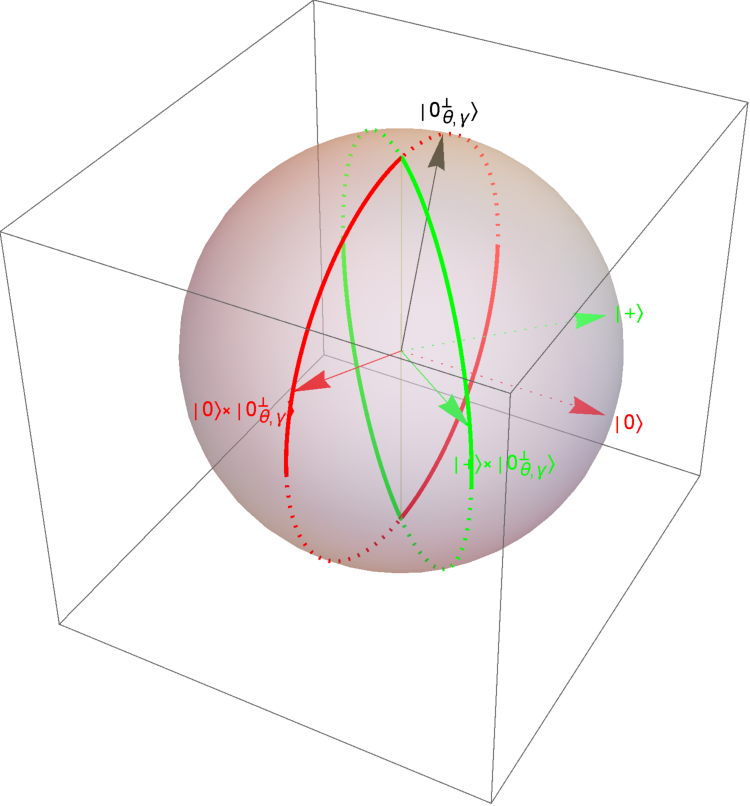
\includegraphics[scale=0.38]{measure4.pdf}
\end{center}
\caption{\label{fig:three-dimensional-4-value}This figure illustrates
  cases 1 and 2 of example~\ref{ex:three-dimensional-4-value} plotted
  in $\mathbb{R}^{3}$. The red and green dotted vectors are $\ket{0}$
  and $\ket{\ps}$ respectively.  All possible real vectors of the subspaces
  $\ket{0_{\theta,\gamma}^{\perp}}$ and
  $\ket{\ps_{\theta,\gamma}^{\perp}}$ are drawn in the red and green
  circles, respectively. Within the circles, a dotted
  vector~$\ket{\psi}$ means $\bar{\mu}(\proj{\psi})=\likely$;
  otherwise, $\bar{\mu}(\proj{\psi})=\unlikely$. The gray vector is a
  generic vector~$\ket{0_{\theta,\gamma}^{\perp}}$, and the red and
  green solid vectors are normalized
  $\ket{0}\times\ket{0_{\theta,\gamma}^{\perp}}$ and
  $\ket{\ps}\times\ket{0_{\theta,\gamma}^{\perp}}$, respectively, where
  $\times$ is the usual cross product in $\mathbb{R}^{3}$}
\end{figure}

Looking closely at the example above, we might think that the
probability measure $\bar{\mu}$ is induced by the state $\ket{2}$
because $\bar{\mu}(\proj{0})=\bar{\mu}(\proj{\ps})=\imposs$, or we
might think it is induced by the state $\ket{1}$ because
$\bar{\mu}(\proj{0})=\bar{\mu}(\proj{\ps'})=\imposs$, or yet we might
think it is induced by the mixed state $\frac{\mathbb{1}}{3}$ because
$\bar{\mu}(\proj{\phi})\ne\necess$ for all $\ket{\phi}$. Each of these
possibilities is compatible with some but not all of the
observations. All is not lost however: if the observations are made
more precise, we conjecture that some of the inconsistencies
disappear. A partial proof of this conjecture is the following example
which refines the previous probability measure by adding more precise
intervals. It remains to prove that this refined measure is convex,
however. 

\begin{example}[Three-dimensional quantum four-interval-valued 
  probability measure]\label{ex:three-dimensional-4-value}
  Given a three dimensional Hilbert space with an orthonormal basis
  $\left\{ \ket{0},\ket{1},\ket{2}\right\} $.  Let \emph{
  }$\mathscr{I}=\left\{ \imposs,\unlikely,\likely,\necess\right\} $,
  $\ket{\ps}=\frac{1}{\sqrt{2}}(\ket{0}+\ket{1})$, and
  $\ket{\ms}=\frac{1}{\sqrt{2}}(\ket{0}-\ket{1})$. The definition of
  $\bar{\mu}$ below refers to Fig.~\ref{fig:three-dimensional-4-value}
  which plots the 1-dimensional projectors:
\begin{enumerate}
\item Let:
\begin{eqnarray*}
\bar{\mu}(\mathbb{0})=\bar{\mu}(\proj{0})=\bar{\mu}(\proj{\ps}) 
  &=& \imposs \\
\bar{\mu}(\mathbb{1})=\bar{\mu}(\mathbb{1}-\proj{0})=\bar{\mu}(\mathbb{1}-\proj{\ps}) 
  &=& \necess
\end{eqnarray*}
where $\ket{0}$ and $\ket{\ps}$ are plotted as the red and green dotted
vectors, respectively.
\item The red and green circles are are the states orthogonal to
  $\ket{0}$ and $\ket{\ps}$, respectively, and can be parametrized as
  $\ket{0_{\theta,\gamma}^{\perp}}=\rme^{\rmi\gamma}\sin\theta\ket{1}+\cos\theta\ket{2}$
  and
  $\ket{\ps_{\theta,\gamma}^{\perp}}=-\rme^{\rmi\gamma}\sin\theta\ket{\ms}+\cos\theta\ket{2}$,
  where $0\le\theta\le\frac{\pi}{2}$ and $0\le\gamma<2\pi$. The dotted
  half of those states need special treatment, i.e., whenever
  $0\le\theta<\frac{\pi}{2}$ and $0\le\gamma<\pi$, we define
\begin{eqnarray*}
\bar{\mu}\left(\proj{0_{\theta,\gamma}^{\perp}}\right)=\bar{\mu}\left(\proj{\ps_{\theta,\gamma}^{\perp}}\right)
  &=& \likely \\
\bar{\mu}\left(\mathbb{1}-\proj{0_{\theta,\gamma}^{\perp}}\right)=
  \bar{\mu}\left(\mathbb{1}-\proj{\ps_{\theta,\gamma}^{\perp}}\right) 
  &=& \unlikely
\end{eqnarray*}
\item Otherwise, $\bar{\mu}(\proj{\psi})=\unlikely$ and $\bar{\mu}(\mathbb{1}-\proj{\psi})=\likely$. 
\end{enumerate}
It is straightforward but tedious to check that $\bar{\mu}$ is a
quantum interval-valued probability measure. Although we have not
verified that $\bar{\mu}$ is convex, the following argument
establishes that is has an empty core. Assume there is a real-valued
probability measure satisfying $\mu_{\rho}^{B}(P)\in\bar{\mu}(P)$ for
all $P\in\events$. Because
$\mu_{\rho}^{B}(\proj{0})\in\bar{\mu}(\proj{0})=\imposs$ and
$\mu_{\rho}^{B}(\proj{\ps})\in\bar{\mu}(\proj{\ps})=\imposs$, we must
have $\mu_{\rho}^{B}(\proj{0})=\mu_{\rho}^{B}(\proj{\ps})=0$ so that
$\mu_{\rho}^{B}=\mu_{\ket{2}}^{B}$. However,
\[
\mu_{\ket{2}}^{B}(\proj{2})=1\notin\unlikely=\bar{\mu}(\proj{2})\textrm{ .}
\]
This measure however is ``better'' than the previous one in the sense
that it might only be induced by $\ket{2}$ or the density matrix
$\frac{\mathbb{1}}{3}$, but not by
$\ket{1}$. 
\end{example}

In general, we conjecture that if the measurement equipment is made
more and more precise, the corresponding interval-valued probability
measure will be closer and closer to the Born rule. In the limit case,
$\mathscr{I}=\left\{ \left\{ a\right\}
  ~\middle|~a\in\left[0,1\right]\right\}$
we do indeed recover the conventional Gleason's theorem and the Born
rule.

\paragraph*{Research Question.} Confirm that as the number and
precision of the intervals increase the quantum interval-valued 
probability measure converges to the measure induced by the Born
rule. 

%%%%%
\subsection{Proposed Activity III: Quantum Information Theorems} 

The previous research question is essentially concerned with the
status of Gleason's theorem in a world with finite-precision
measurements. The following research questions are therefore natural
follow-up questions. 

\paragraph*{Research Question.} Investigate the status of the theorems
of Gleason, Bell, and Kochen-Specker for quantum interval-valued
probability measures. Revisit the Meyer-Mermin debate and its
generalizations in this mathematical framework.

%%%%%
\subsection{Proposed Activity IV: Computational Aspects}

The marriage of quantum mechanics and computer science first
envisioned and popularized by Feynman has created an awkward, but
opportune, moment. The embarrassing dilemma was concisely described by
Aaronson as follows. Consider the following three statements:
\begin{enumerate}
\item[(A)] Textbook quantum mechanics is correct.
\item[(B)] There does not exist an efficient classical factoring
  algorithm.
\item[(C)] The extended Church-Turing thesis that probabilistic Turing
  machines can efficiently simulate any physically realizable model of
  computation is correct.
\end{enumerate}
There is overwhelming evidence to support each of these
statements. The theoretical framework of quantum mechanics (A) has
withstood decades of experimental confirmation. Entire industries are
founded on the assumption (B) that algorithms like RSA are secure and
they also have withstood years of attempted attacks. Finally the
entire field of complexity theory in computer science which has also
withstood years of field testing rests, in essence, on assumption
(C). And yet one of these three statements \emph{must be false}! Indeed
if textbook quantum mechanics is false we concede (A). If it is
correct Shor's efficient factoring algorithm is realizable. If there
is a corresponding efficient classical factoring algorithm then we
concede (B). If not then we concede~(C).

It is unlikely that there will be a simple a resolution to this
awkward situation. It is more likely that the resolution will emerge
from deep and careful analyses of the foundations of each field. In
previous work, we examined the Hilbert space mathematical framework of
quantum mechanics and teased apart its various aspects that directly
rely on the infinite-precision real or complex numbers. We note two
remarkable earlier results:
\begin{itemize}
\item UNIQUE-SAT: Schumacher and
  Westmoreland~\cite{Schumacher2012-SCHMQT} argue that much of the
  structure of traditional quantum mechanics is maintained in the
  presence of finite fields. In particular, they establish that the
  quantum theory based on the finite field of booleans retains the
  following characteristics of quantum mechanics: the notions of
  superposition, interference, entanglement, and mixed states of
  quantum systems; the time evolution of quantum systems using
  invertible linear operators; the complementarity of incompatible
  observables; the exclusion of local hidden variable theories and the
  impossibility of cloning quantum states; and the presence of natural
  counterparts of quantum information protocols such as superdense
  coding and teleportation. However we have argued that this theory is
  not physically realizable as it allows the solution of
  computationally difficult problems like
  UNIQUE-SAT~\cite{Valiant198685} in constant time~\cite{usat}.

\item Deutsch-Jozsa: In a follow-up paper~\cite{DQT2014}, we proposed
  a variant of quantum mechanics in which the underlying field of
  complex numbers is replaced by special finite fields with enough
  structure to model Hermitian products that \emph{locally} behave
  like inner products. The trick is to recognize that, as the
  characteristic of the finite field increases, larger and larger
  regions of the finite field become totally ordered, thereby
  restoring, with some restrictions, all the usual properties of the
  inner product needed for conventional quantum mechanics. Using this
  theory to analyze the Deutsch-Jozsa algorithm reveals that the
  characteristic of the finite field plays an essential role: as the
  size of the finite field grows, so does the numerical range of the
  intermediate and final results of the algorithms being implemented.
  The theory naturally recovers a deterministic measure of the
  intrinsic resources required for a given level of complexity; this
  measure is normally completely hidden in computations with real
  numbers, and explicitly exposing it is one of the significant
  achievements of our discrete field analysis of quantum computation.
  This solves the conundrum that the conventional Deutsch-Jozsa
  algorithm mysteriously continues to work for larger and larger input
  functions without any apparent increase in resources.  Our analysis
  of this problem reveals that as the size of the input increases, it
  is necessary to increase the size of the finite field and hence the
  size of the underlying available numeric coefficients.  This
  observation does not fully explain the power of quantum computing
  over classical computing, but at least it explains that some of the
  power of quantum computing depends on increasingly larger precision
  in the underlying field of numbers.

\end{itemize}

\paragraph*{Research Question.} A long term, ultimate, goal of this
research proposal would be to combine the various pieces into a
coherent computational model of quantum mechanics that keeps explicit
track of resources needed to represent the interactive system
representing the quantum state, its evolution, the observables, and
the probabilities. Such a computational model of quantum mechanics
would encompass classical (reversible) computation and potentially
revolutionize quantum thinking with finite resources. The explicit
manipulation of resources enables one of key idea that emerged in our
previous work: the resources used to represent the quantum system are
in principle unrelated to the resources available to the various
observers. We conjecture that this asymmetry may prove key to
resolving some of the quantum paradoxes.

The nature of quantum mechanics realized in terms of discrete fields
and finitely-communicable probability estimates is amenable to direct
computational exploration for reasonable field sizes and observational
accuracy. We have established a set of utility libraries in
Mathematica that supports a wide variety of such numerical
experiments. Concurrently to this effort, we are also building on our
previous
work~\cite{VDS2009,AGVS2007,AGVS2005,VAS2006,finiteQC,Sabry:2003:MQC:871895.871900}
to build semantically well-founded implementations of the
computational models investigated in this proposal.  The aim of these
implementations is two-fold: (i) to provide an experimental testbed to
simulate physical phenomena (e.g.~\cite{OrtizEtAl2001,SommEtAl2002})
that complements the Mathematica libraries in which quantum algorithms
can be simulated; and (ii) to establish connections between quantum
programming concepts and classical programming concepts.  We plan to
make our software available for educational and research purposes.

\begin{figure}
\begin{center}
  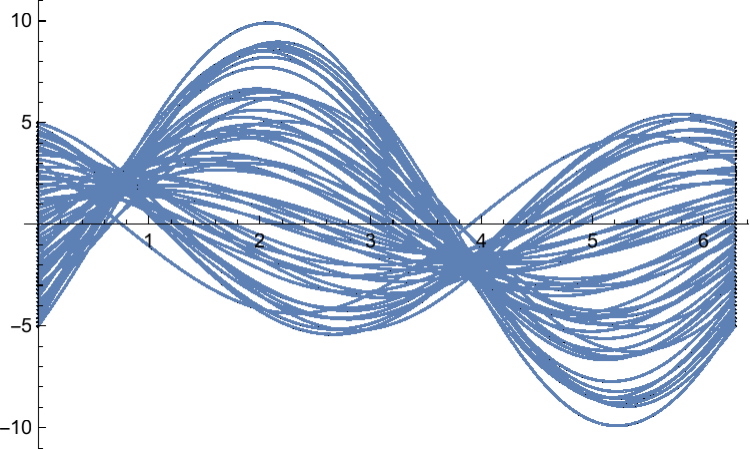
\includegraphics[scale=0.38]{HoughLineData.pdf}
\end{center}
  \caption{Curves of possible line parameters determined by noisy
    data samples on a straight line in 2D space.}
\label{houghline.fig}
\end{figure}

%%%%%
\subsection{Proposed Activity V: Applications}

A classic evidence-accumulation method known as the Hough
transform~\cite{BallardGenHough1981}, which is very closely related to
Bayesian evidence accumulation
methods~\cite{CrandallEtal2005,CrandallEtal2006}, provides another
example of how our proposal to define physical theories without exact
real numbers could be combined with the measurement process. Simply
described, the Hough transform as an abstraction of Bayesian schemes
starts with a model of the theory being measured, typically a model
that would ordinarily be treated {\it after\/} gathering the data by
applying least squares to choose the optimal parameters.  But in this
method, instead of thinking of, say, the model of a straight line
$\hat{\mathbf{n}}\cdot \mathbf{x} = d$ as an equation for the points
on a line $ \mathbf{x}_{i} = (x_{i},y_{i})$, we think of it as a
time-accumulating {\it set\/} of equations for the distance $d$ of the
nearest point on the line and the direction
$ \hat{\mathbf{n}} = (\cos \theta, \sin \theta)$ from the origin to
that point (the direction perpendicular to the line).  Thus each point
of {\it evidence\/}, $(x_{i},y_{i})$, produces an {\it equation in the
  parameter space\/} that is effectively a plot of all the possible
values of $d(\theta)$ as a function of the possible angular directions
$\theta$ pointing to the family of all possible lines.  A typical
result from a set of errorful (it is impossible to measure real
numbers, we recall) data measurements of points on a hypothetical
straight line is shown in Fig.~\ref{houghline.fig}.

The interesting step for us is now to realize that the {\it parameter
  curves\/} shown in the figure do not need, or indeed, must not, be
themselves infinitely precise real numbers, but they must themselves
incorporate in some way a theory consistent with forbidding absolute
precision.  In practice, then, the sinusoidal lines in Figure
\ref{houghline.fig} all become fuzzy, and the accumulation of these
fuzzy distributions produces peaks of likelihood around the values
$(d_0, \theta_0)$ that are the optimal choices for the line describing
the set of data.  Note that even {\it one\/} data point provides
evidence on a set of hypotheses. The simple analysis we have outlined
here is easily extended to much more complex situations in higher
dimensions (see, e.g.,~\cite{BallardGenHough1981}).  Our point here is
that essentially any physical theory that would ordinarily be
described by a mathematical model using infinite precision numbers is
potentially nonsensical from a computational point of view: computer
scientists know perfectly well, and have been dealing with since the
time of Turing and Shannon, that every single bit of precision in any
number has a cost, and that there is not enough energy in the universe
to compute even one general real number.  Thus the combination of
physical models that, in some intrinsic fashion, contain only
computable numbers, with theories of measurement and evidence in the
fashion of the Hough transform example we have just presented, could
contain the outline of entirely new ways of understanding what
mathematical models of the physical world and its measurement actually
could be.

%%%%%%%%%%%%%%%%%%%%%%%%%%%%%%%%%%%%%%%%%%%%%%%%%%%%%%%%%%%%%%%%%%%%%%%%%%%%%%
\section{Broader Impact and Education} 

\noindent (A) {\em Integration of research and education:} Courses on
advanced computational models and quantum information will be further
developed at Indiana University to communicate the basic concepts and
tools discussed in this proposal. Dr. Ortiz taught courses on
``Quantum information and Computation'' and Dr. Sabry has taught
courses on ``Quantum Computing'' for graduate students.  Dr.\ Hanson
has taught courses on scientific visualization and mathematical
modeling with emphasis on high-dimensional mathematics.  His numerous
Siggraph course presentations are embodied in his 2006 book {\it
  Visualizing Quaternions\/}, which remains the definitive treatment
of the subject for computer science and data analysis applications and
has sold thousands of copies. As a part of Dr.\ Hanson's commitment to
exposing and explaining the elements of higher mathematics to the
public, he has recently led the design of a free iPhone App, {\it
  4Dice\/}, that for the first time makes available an interactive
treatment of a correctly imaged simulation of the appearance of a
hypercube, realizing interactively his YouTube animation of the same
name.  This framework is now being generalized for a broad family of
iPhone Apps to permit the hands-on study of high-dimensional
mathematics.  These courses were highly appreciated by the students as
noted by their evaluations in making the material extremely accessible
and interesting.  The PIs plan to engage high school students or
undergraduates in the implementation of some of the ideas.  The PIs
have a long standing commitment to K-12 science and math education
(see also (C) below). The collaborative group efforts will provide
students, as well as the PIs with a unique learning experience. The
broadened perspectives gained through those efforts will contribute to
the PIs effectiveness as teachers and mentors. They also will enable
to better prepare students and postdocs for productive careers in an
increasingly competitive global economy. Students and postdocs are
encouraged to pursue collaborative research leading to a broader
scientific program. This is highlighted by the PIs students' close
contact with LANL, the Perimeter Institute, and the Institute for
Quantum Computing at Waterloo.

\medskip
\noindent (B) {\em Broadening the participation of underrepresented groups:}
Indiana University is engaged in attracting women and minorities in all
ranks. Several programs are aimed at specifically attracting outstanding
students into physics and computer science, and to expanding the pool of
candidates for fellowships. Targeted recruitment of minority graduate
students is facilitated by the Falicov Fellowship established in 2006. In
recent years, the School of Informatics and Computing has been fortunate to
hire several women and minorities for faculty positions, and we have been
working toward increasing the number of women and minorities among our
student population. To assist with this process, the PIs will encourage women
and minorities to apply for graduate positions as well as undergraduate
positions that may be made available by the grant and REU
supplements. Dr. Ortiz has minority students and Dr. Sabry has graduated a
female Ph.D. in 2005 and is currently assisting on the Ph.D. committees of
several others. 

\medskip
\noindent (C) {\em Enhancing infrastructure and outreach:} Dr. Ortiz
has pursued broad outreach by giving talks on astronomy/astrophysics
in the local schools at Bloomington, Indiana, and by an interview in
the public radio on quantum information. Dr. Ortiz is also guiding a
high school student in work on interferometry in two and three slit
experiments. Dr. Ortiz also guides undergraduate research. All source
code produced by this project will be made freely available via the
web, and the results will be disseminated via technical reports,
conference papers, and journal articles.  The software and concepts we
have developed in the past have been employed by a wide variety of
commercial and noncommercial users.  Thus, we expect that the
successful completion of the proposed research will contribute to the
understanding of quantum and semi quantum computation. The educational
benefits that will flow from this proposal will extend beyond the
students of the participating research groups. The knowledge gained
through participation in the proposed research will further strengthen
the effectiveness of these outreach activities.

%%%%%%%%%%%%%%%%%%%%%%%%%%%%%%%%%%%%%%%%%%%%%%%%%%%%%%%%%%%%%%%%%%%%%%%%%%%%%%
\section{PI Team and Prior NSF Support} 

\paragraph*{PI Team.} Over the past several years, the PIs, together
with other IU faculty members and students, have formed a group whose
main interest is the study of paradigms of computing that either arise
in nature or are inspired by natural phenomena. The PIs are especially
interested in how the laws of physics can inspire and guide our
abstract computational models, as well as exposing new insights into
the computational framework behind the natural world and the
computability of physical theory. Our group has been active in several
areas related to the theory behind quantum computation. Particular
areas include: mathematical foundations of quantum computation and
complexity~\cite{AGVS2007,VAS2006}, adiabatic quantum computing,
quantum logic, classical and quantum reversible programming
languages~\cite{Sabry:2003:MQC:871895.871900}, analog computation and
its limits, and optical computing. During the past several years, our
discussions have revolved around formulating variants of quantum
mechanics that are computable and that are as close to possible to
classical computing. Several preliminary results have emerged from our
collaboration~\cite{usat,finiteQC,geometry2013,DQT2014}, and the group
is very excited about the potential implications of those
results. This proposal brings forth a particular aspect of this
programme related to its applications to problem areas that have
traditionally been outside the conceptual framework of quantum
mechanics and programming language research. This proposal, if funded,
will give our group more recognition within the university which, at
this point, is committed to generously funding several ``emerging
areas of research''. With the establishment of a new Intelligent
Systems Engineering at Indiana University with a focus nanoscale
sensors and quantum engineering and the recent hires in Physics in
experimental atomic physics, ion-trap quantum simulation, computation,
and measurement, the PI group is in an excellent position to receive
additional funding from the University to reach a critical mass of
quantum information researchers.

\paragraph*{Prior Support.} There was no recent NSF support for
Dr. Ortiz or Dr. Hanson. In the past five years, Prof. Sabry received
one NSF grant (award number 1217454) titled \emph{Information Effects}
for the amount of \$275,319.00 with start and end dates of 1 September
2012 -- 31 August 2016.

\paragraph*{Intellectual Merit.} Computing is about processing
information. Physically speaking, information, like energy, is a
resource that obeys a conservation principle: information can never be
created nor destroyed; it is just transformed. Traditional models of
computation, however, have not embraced this conservation of
information as an explicit principle. Instead this principle appears,
after the fact, in applications such as information-flow security
which treats the amount of information released to the environment as
a possible security leak and such as differential privacy which
intentionally releases some random information to the user to confuse
potential attackers. This project has instead embraced the principle
of conservation of information as a key foundation for the design of
computational models. In one perspective, computation in these models
is constructed from reversible transformations that act on topological
spaces, deforming them, stretching them, and shrinking them but never
cutting nor glueing. The first main result of this project was the
design and implementation of a programming language which captures
these ideas and realizes them in the context of the new foundational
framework of Homotopy Type Theory. This framework combines ideas from
mathematics, logic, physics, and computation in a way that accounts
for a newly-recognized higher-dimensional structure of types. This
idea enabled us to not only represent programs as reversible
deformations but also to represent the reversible deformations
themselves as higher-level programs implementing reversible
optimizations of the underlying lower-level programs. In a second
breakthrough, viewing the higher-level programs as distinct proofs of
reversibility enabled the definition of types whose natural
cardinality is fractional. Having computations that manipulate
fractional types opens the door for a rich and novel class of
applications in which resource creation and resource use are
separated. This idea brings speedups and convenience in a way that is
similar to the speedup and convenience brought by the use of credit
cards to complete transactions without necessarily having the money at
hand: the monetary resource can be consumed by the merchant and only
later be reconciled by the buyer.

\paragraph*{Broader Impacts.} The idea of reversible computation and
its connection to quantum mechanics is at the heart of one of the
deepest mysteries in the universe. Any progress or theory that
explains physical principles computationally is likely to change our
worldview impacting everything from philosophy and religion to all
conventional sciences. On the development of researchers, the project
resulted in the graduation of one Ph.D. student with another one
expected to graduate in Spring 2017, the current supervision of two
additional Ph.D. students, the graduation of an MS student, and the
hosting of a visiting scholar.

\paragraph*{Publications.} Several papers were published to report on
the results. On the foundational side, we have the following papers:
(1) Computing with Semirings and Weak Rig Groupoids, ESOP, 2016, (2)
Superstructural Reversible Logic, Workshop on Linearity, 2014, (3)
Theseus: A High Level Language for Reversible
Computing. Work-in-Progress report, RC 2014, (4) Discrete Quantum
Theories, J. Phys. A: Math. Theor. 2014., (5) Geometry of Discrete
Quantum Computing, J. Phys. A: Math. Theor. 2013., (6) Isomorphic
Interpreters from Logically Reversible Abstract Machines. RC 2012. On
the applications side, we have the following papers: (1) Copredication
in Homotopy Type Theory: A homotopical approach for formal semantics
of natural languages. Workshop on Natural Language and Computer
Science, 2016., (2) Contract Monitoring Semantics as Patterns of
Communication. ICFP, 2015., (3) Extensible Effects: An Alternative to
Monad Transformers. Haskell Symposium, 2013., (4) Encoding Secure
Information Flow with Restricted Delegation and Revocation in
Haskell. Workshop on Functional Programming Concepts in
Domain-Specific Languages, 2013. In addition to the publications,
Dr. Sabry and collaborators maintain a public repository with software
related to the project. Dr. Sabry was also invited to give talks at
several venues, most notably the Colloquiumfest, University of
Saskatchewan, Canada, 2014, and the Workshop on Quantum Information
and Foundations of Quantum Mechanics, University of British Columbia,
Vancouver, Canada, 2013

% (d) a listing of the publications resulting from the NSF award (a
% complete bibliographic citation for each publication must be provided
% either in this section or in the References Cited section of the
% proposal); if none, state "No publications were produced under this
% award."

% (e) evidence of research products and their availability, including,
% but not limited to: data, publications, samples, physical collections,
% software, and models, as described in any Data Management Plan; and

%%%%%%%%%%%%%%%%%%%%%%%%%%%%%%%%%%%%%%%%%%%%%%%%%%%%%%%%%%%%%%%%%%%%%%%%%%%%%%
\newpage
\printbibliography
\end{document}

%%%%%%%%%%%%%%%%%%%%%%%%%%%%%%%%%%%%%%%%%%%%%%%%%%%%%%%%%%%%%%%%%%%%%%%%%%%%%%



